\documentclass[11pt]{article}

\usepackage[margin=1in]{geometry}
\usepackage[T1]{fontenc}
\usepackage{lmodern}
\usepackage{amsmath,amssymb}
\usepackage{booktabs}
\usepackage{tabularx}
\usepackage{array}
\usepackage{enumitem}
\usepackage{microtype}
\usepackage{graphicx}
\usepackage{placeins}
\usepackage{tikz}
\usetikzlibrary{positioning,arrows.meta,fit}
\usepackage[numbers,sort&compress]{natbib}
\usepackage{xurl}
\usepackage[hidelinks]{hyperref}

\setlist{itemsep=2pt,topsep=4pt}
\setlength{\emergencystretch}{1.5em}
\newcolumntype{L}{>{\raggedright\arraybackslash}X}
\newcolumntype{P}[1]{>{\raggedright\arraybackslash}p{#1}}

\title{Fast 4-bit KV-Cache Decoding on Hopper GPUs:\\
Why Existing Kernels Are Slow and How to Fix Them}
\author{Jian Zhang\\ Northeastern University}
\date{November 2026}

\begin{document}

\maketitle

\begin{abstract}
A 4-bit KV cache reads about half the bytes of FP8, but Hopper GPUs have no FP4 hardware and little instruction-issue capacity per byte of memory bandwidth, so the 4-bit values must be decoded in software within a tight budget. On H200, FlashInfer's NVFP4 decode, the kernel behind vLLM's NVFP4 KV path on Hopper, reaches only 10--20\% of memory bandwidth and is up to 1.7$\times$ slower than FP8. NVBit instruction counts show two separate causes: the Triton and FlashInfer kernels execute two to three times Hopper's issue budget per byte, and the kernels we counted serialize loading, decoding and matrix multiplies. We build a Hopper-native decode kernel that overlaps a TMA producer warp with two compute warpgroups, lays the cache out at write time so that decoded values feed the tensor cores from registers, and swaps the matrix operands so that small query groups need no padding rows. On H200 it reaches 67--75\% of peak bandwidth at batch 32--128 and at all 11 shapes is faster than both FP8 decode kernels we measured, 1.2--2.1$\times$ faster than FlashInfer's XQA. Inside vLLM, with an accuracy recipe (K mean removal, K rotation, four BF16 sink tokens, a BF16 first layer), it decodes 1.12--1.64$\times$ faster per step than vLLM's FlashInfer FP8 path at batch 8 and above, is level at batch 1, and holds 1.63$\times$ as many tokens. On one H200 under a reasoning-like request stream, the highest rate at which 99\% of requests meet the latency targets is 1.23--1.32$\times$ FP8's on Llama-3.1-8B, 1.45--1.80$\times$ on Qwen3-32B and 1.67--2.20$\times$ on Qwen2.5-72B, as the cache becomes the limit; prefill-heavy streams are worse with ours (7\% slower prefill). On five models from 7B to 32B, repeated runs show no significant accuracy difference from BF16 KV. We also link the collapse of Qwen2-family reasoning models under FP8 KV to the layer-0 key bias identified by prior work, and show that keeping that layer in BF16 restores both FP8 and 4-bit KV.
\end{abstract}

\section{Introduction}
\label{sec:intro}

In long-context and batched serving, every decoding step reads the whole KV cache, so decode attention is limited by memory bandwidth. For Llama-3.1-8B (32 query heads, 8 KV heads, head dimension 128), each KV row of 256 bytes in BF16 feeds about 1,024 floating-point operations, roughly 4 per byte, while an H200 can do about 206 dense BF16 tensor-core operations per byte (989 TFLOPS $\div$ 4.8 TB/s, spec-sheet values). Time per step is therefore close to bytes read divided by bandwidth, and fewer bytes means faster decoding and more requests per GPU.

NVIDIA's Blackwell GPUs decode 4-bit formats such as NVFP4 in hardware. The installed base is still largely Hopper (H100, H200, H20), which supports BF16 and FP8 but not FP4. There, 4-bit values must be unpacked and scaled in software inside the attention kernel. We measured what that costs today: at batch 32 and 16K context on H200, FlashInfer~\cite{ye2025flashinfer} takes 0.495 ms in BF16, 0.395 ms in FP8 (0.255 ms with its XQA kernel, measured in a separate job) and 0.669 ms in NVFP4. A vLLM~\cite{kwon2023vllm} user who enables an NVFP4 KV cache on Hopper saves memory but decodes more slowly.

That software decoding can make low-bit attention compute-bound was argued by QServe~\cite{lin2025qserve} for INT4 on A100. Hopper makes the problem harder: its memory bandwidth grew faster than its instruction issue rate, so the number of instructions a kernel may spend per byte at full bandwidth is smaller (Section~\ref{sec:stall}).

Contributions:

\begin{enumerate}
  \item \textbf{Diagnosis by measurement.} Using NVBit~\cite{villa2019nvbit} instruction counts against Hopper's issue budget (about 7 thread instructions per byte at full bandwidth on H200), we show that existing 4-bit decode kernels stall for two separate reasons, too many instructions and serialized waiting, and that different kernels stall for different ones.
  \item \textbf{A Hopper-native 4-bit decode kernel} for NVFP4, MXFP4 and INT4, with paged KV support for the FP4 formats. At the kernel level on H200, NVFP4 is 1.2--2.1$\times$ faster than FlashInfer's XQA FP8 kernel and 1.4--2.3$\times$ faster than its FA2 FP8 kernel. The pipeline structure follows FlashAttention-3 and LiquidGEMM. None of its parts is new on its own: swapping the A and B operands for a small M is common in GEMM kernels (e.g.\ vLLM's SM90 FP8 GEMM~\cite{vllm20396}), and BitDecoding-FP4~\cite{du2026bitdecodingfp4} swaps the operands of both attention matrix multiplies for FP4 KV decoding on Blackwell's native FP4 tensor cores; BitDecoding~\cite{du2025bitdecoding} packs low-bit KV in a tensor-core-aware layout, Marlin~\cite{frantar2024marlin} reorders 4-bit weights offline so that each thread's fragment is contiguous, TensorBridge~\cite{zou2026tensorbridge} combines the operand swap with offline-permuted NVFP4 weights to feed Hopper's FP8 wgmma from registers, FuTransformer~\cite{wang2026futransformer} stores an INT4 copy of K in mma.sync fragment order on H100, and FServe~\cite{baek2026fserve} decodes an INT4 KV cache to FP8 in registers for FlashAttention-3-based kernels on H100, with decode speed competitive with, or above, FlashAttention-3's FP8 kernel in its measurements (it does not compare with XQA). What we add is their use in decode attention over E2M1 (NVFP4, MXFP4) as well as INT4 KV caches on Hopper, which has no FP4 hardware, faster than the FP8 decode kernels we measured: the cache-write kernel lays out the cache online so that each thread's fragment is contiguous, decoded K and $V^\top$ both feed wgmma from registers, and the swap keeps small query groups free of padding rows; the instruction counts of Section~\ref{sec:stall} show why these choices are needed within Hopper's issue budget.
  \item \textbf{End-to-end results in vLLM} through a plugin, against FlashInfer FP8 with the XQA decode kernel (the faster of the two FP8 backends we measured in vLLM, and the kernel vLLM's FlashInfer backend selects on Hopper when its artifact check succeeds) and against vLLM's own NVFP4 KV path, including the highest request rate one GPU sustains under load: 1.23--1.32$\times$ FP8's on Llama-3.1-8B, growing to 1.67--2.20$\times$ on Qwen2.5-72B as the KV cache becomes the limit (Table~\ref{tab:capacity}).
  \item \textbf{An accuracy recipe, and a known mechanism linked to a serving failure:} K mean removal is needed for small-group FP4 on some models. Liu et al.~\cite{liu2025quantreasoning} traced the K outliers of R1-Distill-Qwen models to the key-projection bias inherited from their Qwen base models and studied 3- and 4-bit KV; we connect this mechanism to the reported collapse of Qwen2-family reasoning models under FP8 KV~\cite{li2025rllmserving}, which we reproduce in vLLM 0.33, show that keeping only layer 0 in BF16 fixes both FP8 and 4-bit KV, and add a control: the same R1 distillation on a Llama base, which has no key bias, does not collapse.
  \item \textbf{Findings reported to vLLM} (Appendix~\ref{sec:vllm}): a scale constant in its UltraQuant format, the layer-0 FP8 failure, a prefix-cache correctness bug, and which proposed eval checks catch such bugs.
\end{enumerate}

\paragraph{Practical notes for vLLM users on Hopper.} From our measurements (vLLM 0.33, Llama-3.1-8B unless noted, H200):
\begin{itemize}
  \item vLLM's NVFP4 KV cache (\texttt{-{}-kv-cache-dtype nvfp4}) saves memory but decodes 1.4--2.3$\times$ slower than FP8 at batch 8 and above and about 1.1$\times$ slower at batch 1 (Section~\ref{sec:e2e}). Its UltraQuant format falls back to Triton decode kernels on NVIDIA and is 1.8--3.9$\times$ slower than FP8 per step.
  \item With FlashInfer and FP8 KV, vLLM uses the faster XQA decode kernel only if its network check to NVIDIA's artifact server succeeds; when the check fails (on our cluster, behind a proxy), it falls back to FlashInfer's own decode kernel without an error. Check the log for \texttt{decode\_backend=xqa} (Section~\ref{sec:background}).
  \item Qwen2-family reasoning models can collapse under FP8 KV without any error. Keeping layer 0 in BF16 (\texttt{-{}-kv-cache-dtype-skip-layers 0}, 1/28 more KV memory on a 28-layer model) restored them in our runs (Section~\ref{sec:accuracy}), but skipping layers crashes FlashAttention-3 for some models (\#65821~\cite{vllm65821}; fix proposed in \#65891~\cite{vllm65891}).
  \item Our plugin helps most when decoding dominates and KV memory is the limit (batch 8 and above, long outputs, large models on one GPU; Table~\ref{tab:capacity}). At batch 1 it is level with FP8, and prefill-heavy streams are slower (Section~\ref{sec:e2e}). It supports head dimension 128 with up to 8 query heads per KV head (Section~\ref{sec:limits}).
\end{itemize}

\section{Background and related work}
\label{sec:background}

\paragraph{Notation.} $B$ is the number of sequences in a decode batch and $S$ the context length in tokens. A \emph{row} is one token's K (or V) for one KV head: 128 values. $G$ is the number of query heads per KV head (4 for Llama-3.1-8B). Decode kernels split each sequence into chunks processed in parallel and combine the partial results in a \emph{split merge}, as in Flash-Decoding~\cite{dao2023flashdecoding}. \emph{Sink tokens} are the first four tokens of each sequence, which we keep in BF16 outside the 4-bit cache~\cite{xiao2023streamingllm,liu2024intactkv}. The \emph{recipe} is NVFP4 with K mean removal, Hadamard rotation of K, four BF16 sinks and layer 0 in BF16.

\paragraph{Formats.} Table~\ref{tab:formats} lists the formats per row.

\begin{table}[tbp]
\centering
\caption{Formats, per 128-value head row.}
\label{tab:formats}
\small
\begin{tabularx}{\linewidth}{@{}llLr@{}}
\toprule
Format & Element & Scale & Bytes per row \\
\midrule
BF16 & 16-bit float & none & 256 \\
FP8 (E4M3) & 8-bit float & per tensor & 128 \\
INT4 (per token, asymmetric) & 4-bit integer & FP16 scale and zero point per row & 68 \\
NVFP4 & E2M1 & E4M3 per 16 values, plus a per-tensor FP32 scale & 72 \\
MXFP4 / UltraQuant & E2M1 & E8M0 (power of two) per 32 values & 68 \\
\bottomrule
\end{tabularx}
\end{table}

\paragraph{Fast low-bit decode kernels.} QServe~\cite{lin2025qserve} showed that a naive INT4 KV attention kernel can be slower than an INT8 one on A100 because dequantization on CUDA cores exceeds the roofline in operations per byte, and made it up to 1.5$\times$ faster than an INT8 kernel with cheaper bit manipulation, FP16 instead of FP32 arithmetic and prefetched scales; it reports no Hopper results. The magic-number conversion of integers to FP16 that QServe, Marlin~\cite{frantar2024marlin} and our INT4 path use is described by Kim et al.~\cite{kim2022elephants}. On H100, PyTorch's INT4 GQA decode kernels reach 17--30\% of bandwidth after extensive tuning, against 44--64\% for BF16 (our arithmetic from the reported GB/s)~\cite{pytorch2024int4decoding}. FOSCAR~\cite{zhuang2026foscar} introduced affine folding for INT4 KV decoding and reports near-peak bandwidth on H100; its instruction-budget argument (its Eq.~2) is the model we use in Section~\ref{sec:stall}. BitDecoding~\cite{du2025bitdecoding} decodes INT4 KV on Hopper with TMA, warp specialization and wgmma; its packing keeps a tensor-core-aware layout, and on Hopper it writes the dequantized values to shared memory for wgmma. BitDecoding-FP4~\cite{du2026bitdecodingfp4} targets Blackwell's native FP4 tensor cores (B300 and RTX PRO 5000 in its experiments); it swaps the two attention matrix multiplies to compute the transposed score and probability tiles. NVFP4-MLA~\cite{ni2026nvfp4mla} stores and computes multi-head latent attention in NVFP4 on Rubin GPUs. LiquidGEMM~\cite{hu2025liquidgemm} uses one load warpgroup and two compute warpgroups that dequantize in registers and feed wgmma directly, for W4A8 GEMM on Hopper; our kernel applies the same structure to attention, where a softmax sits between the two matrix multiplies. FlashInfer provides the BF16, FP8 and NVFP4 decode paths vLLM uses on Hopper. FuTransformer~\cite{wang2026futransformer} fuses a Llama decode block on H100 with an INT4 copy of a BF16 KV cache: K is stored in mma.sync fragment order and filled into registers through a shared-memory lookup table, per-token scales are applied after the QK dot product, and V is transposed through shared memory; it is compared with PyTorch baselines, not with production FP8 KV attention kernels. FServe~\cite{baek2026fserve} (following FireQ~\cite{baek2025fireq}) stores an INT4 KV cache with per-token group scales, quantizes q to FP8 and dequantizes K and V to FP8 in registers, so that its FlashAttention-3-based prefill and decode kernels run on FP8 wgmma; it is integrated into vLLM and measured on H100. Its decode kernel reaches an effective (BF16-equivalent) bandwidth competitive with, or above, FlashAttention-3 with an FP8 cache (its Figure 7), and in a profile of 132 variable-length requests both take 1.52 ms (its Table 4); it is not compared with XQA. Ours differs in the formats (E2M1 with block scales as well as INT4), in feeding the decoded values to FP16 wgmma as the register operand with the operands swapped, and in the write-time layout. TensorBridge~\cite{zou2026tensorbridge} runs NVFP4 weights on Hopper's FP8 wgmma by computing $Y^\top = W X^\top$ so that the weights are the register operand, with weights pre-permuted for 16-byte fragment loads; it is a weight GEMM, not attention. On AMD MI355X, the UltraQuant paper~\cite{chakrabarti2026ultraquant} finds that 4-bit KV ``buys capacity, not kernel speed'': its decode attention takes 2.45$\times$ FP8's time with software dequantization and 1.18$\times$ with native FP4 (32K context, batch 8). An open vLLM PR (\#53060~\cite{vllm53060}) adds a CUDA 4-bit (TurboQuant) decode path for Hopper and compares it with BF16 FlashAttention and vLLM's existing TurboQuant path, not with an FP8 KV cache. LMDeploy's TurboMind~\cite{lmdeploy} has an INT4 KV cache that is faster than its own INT8 and BF16 caches on H200 (Section~\ref{sec:limits}). Our kernel combines warp specialization (as in FlashAttention-3~\cite{shah2024flashattention3}), write-time layouts (as in Marlin) and folding (as in FOSCAR).

\paragraph{Accuracy of low-bit KV caches.} KIVI~\cite{liu2024kivi} and KVQuant~\cite{hooper2024kvquant} quantize keys per channel because of channel outliers; QuaRot~\cite{ashkboos2024quarot} and SAW-INT4~\cite{jia2026sawint4} rotate K with a Hadamard transform, and SAW-INT4 shows that per-token INT4 needs it. SageAttention's~\cite{zhang2025sageattention} ``smooth K'' subtracts the per-channel mean of K. For INT4 keys, FServe~\cite{baek2026fserve} subtracts an offline-calibrated fraction of the per-channel mean after RoPE (``shrunk centering'') and aligns per-channel ranges with a scale folded into q, and FireQ~\cite{baek2025fireq} combines pre- and post-RoPE scaling. FlagRot~\cite{shao2026flagrot} reports that whole-head Hadamard rotation raises the KL of NVFP4 caches on Qwen3-8B (by 215\%) and that choosing per sub-vector whether to rotate avoids this; BitDecoding-FP4's default recipe on Blackwell includes static key smoothing (a calibrated per-head mean), a Hadamard rotation and the first 16 tokens in BF16, close to ours. Jet-QSparse~\cite{tang2026jetqsparse} likewise combines an NVFP4 cache with calibrated key centering and at most two BF16 pages per sequence and layer on Blackwell (GB300), with FP8 prefill. KVQuant and IntactKV~\cite{liu2024intactkv} keep the first token in high precision. Our accuracy results reproduce these on Hopper and add the layer-0 finding.

\paragraph{Serving.} vLLM 0.33 offers FP8 KV through FlashAttention-3 (default) or FlashInfer (faster than FlashAttention-3 for FP8 KV on H100 in vLLM \#66590~\cite{vllm66590}, and on H200 in our runs), an NVFP4 KV cache decoded by FlashInfer, and a 4-bit UltraQuant format (MXFP4 with K rotation)~\cite{chakrabarti2026ultraquant}. With FlashInfer and FP8 KV on Hopper, vLLM decodes with TensorRT-LLM's XQA kernel, shipped in FlashInfer, but only if a network check to NVIDIA's artifact server succeeds; otherwise it falls back to FlashInfer's own decode kernel without an error. We log the resolved kernel in every run (Section~\ref{sec:setup}). On NVIDIA, UltraQuant falls back to Triton~\cite{tillet2019triton} decode kernels and FlashAttention-2~\cite{dao2023flashattention2} prefill (the latter addressed by vLLM PR \#47531~\cite{vllm47531}). The FP8 baseline is moving: open PRs bring FlashAttention-4's native FP8 to vLLM's SM90 FP8-KV path~\cite{fa206,vllm63139}; we have not measured them.

\section{Why existing 4-bit kernels stall}
\label{sec:stall}

The 4-bit kernels we examined either execute two to three times Hopper's instruction budget per byte, or wait on serialized loads and barriers, or both; reaching bandwidth needs both problems fixed.

\paragraph{Issue budget.} An H200 issues at most about 33 trillion thread instructions per second (132 SMs $\times$ 4 schedulers $\times$ 32 lanes $\times$ 1.98 GHz) and reads 4.8 TB/s, so a kernel running at full bandwidth can spend about 7 thread instructions per byte, or about 3.9 per value at 72 bytes per 128-value row. This follows FOSCAR's Eq.~2. With the same formula and spec-sheet values, the budget is about 10 on H100 SXM and A100 and about 53 on L40S, which is why software 4-bit decoding that pays off on A100 or L40S~\cite{lin2025qserve} can still be issue-bound on H200.

\paragraph{Measured instruction counts.} GPU performance counters were not available on our cluster, so we counted executed instructions with NVBit, NVIDIA's binary instrumentation tool ($B = 32$, $S = 16$K; Table~\ref{tab:nvbit}).

\begin{table}[tbp]
\centering
\caption{Measured instruction counts (NVBit, H200, $B = 32$, $S = 16$K). Implied issue utilization = instructions per byte $\times$ measured bandwidth fraction $\div$ 7.}
\label{tab:nvbit}
\small
\begin{tabularx}{\linewidth}{@{}Lllll@{}}
\toprule
Kernel & Instructions per value & Bandwidth used & Implied issue utilization & Main problem \\
\midrule
Our first Triton NVFP4 kernel & 11.7 & 17\% & 52\% & both \\
FlashInfer NVFP4 & 8.3 & 19\% & 40\% & both \\
BitDecoding INT4 (Hopper branch) & 3.6 without spin-waits & 25\% & about 24\% & waiting \\
\bottomrule
\end{tabularx}
\end{table}

Ours and FlashInfer's exceed the budget two to three times; most extra instructions are integer and bit operations (IMAD, LOP3, PRMT), multiplies and type conversions, plus, in Triton, round trips of decoded values through shared memory (three to five per tile, depending on the Triton version). BitDecoding decodes cheaply (about 1.3 instructions per value) and stays within the budget without its spin-waits, but serializes decoding and the matrix multiply, spends 38\% of executed instructions spin-waiting on barriers, and puts the 4 query heads on wgmma's 64-row dimension, so a third of its useful work is softmax on padding rows. Fixing only the instruction count, or only the overlap, is not enough.

\section{Design}
\label{sec:design}

The kernel fixes waiting with warp specialization and fixes the instruction count by choosing the cache layout at write time; INT4, NVFP4 and MXFP4 share one structure (Figure~\ref{fig:pipeline}).

\begin{figure}[tbp]
\centering
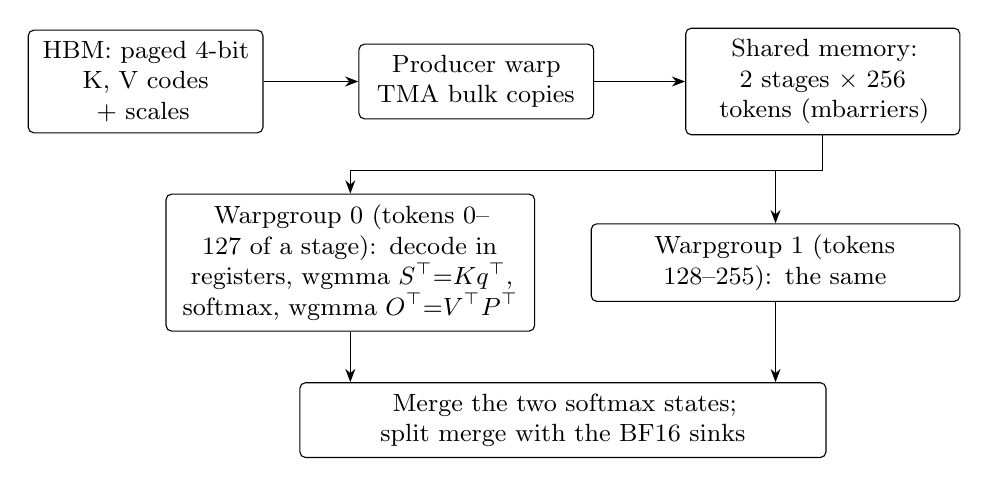
\begin{tikzpicture}[font=\small, box/.style={draw, rounded corners=2pt, align=center, inner sep=4pt}, >=Stealth]
\node[box, text width=2.7cm] (hbm) at (0,0) {HBM: paged 4-bit\\K, V codes + scales};
\node[box, text width=2.7cm] (prod) at (4.2,0) {Producer warp\\TMA bulk copies};
\node[box, text width=3.2cm] (smem) at (8.6,0) {Shared memory: 2 stages $\times$ 256 tokens (mbarriers)};
\node[box, text width=4.4cm] (wg0) at (2.6,-2.3) {Warpgroup 0 (tokens 0--127 of a stage): decode in registers, wgmma $S^\top{=}Kq^\top$, softmax, wgmma $O^\top{=}V^\top P^\top$};
\node[box, text width=4.4cm] (wg1) at (8.0,-2.3) {Warpgroup 1 (tokens 128--255): the same};
\node[box, text width=6.4cm] (merge) at (5.3,-4.3) {Merge the two softmax states; split merge with the BF16 sinks};
\draw[->] (hbm) -- (prod);
\draw[->] (prod) -- (smem);
\draw[->] (smem.south) -- ++(0,-0.45) -| (wg0.north);
\draw[->] (smem.south) -- ++(0,-0.45) -| (wg1.north);
\draw[->] (wg0.south) -- (wg0.south |- merge.north);
\draw[->] (wg1.south) -- (wg1.south |- merge.north);
\end{tikzpicture}
\caption{Kernel structure. Loads, decoding and the two matrix multiplies overlap: while the warpgroups decode and multiply one stage, the producer fills the other. Decoded K and $V^\top$ are wgmma's A operand, read from registers; query heads are the N = 8 dimension.}
\label{fig:pipeline}
\end{figure}

\begin{enumerate}
  \item \textbf{Overlap: a TMA producer and two compute warpgroups.} A producer warp streams 256-token stages of K and V (codes and scales) into shared memory with TMA bulk copies, double-buffered with mbarriers. Each compute warpgroup (4 warps) owns half of every stage and keeps its own online-softmax state; the two merge once at the end.
  \item \textbf{Operand swap, decoded values straight from registers.} QK is computed as $S^{\top} = K \cdot q^{\top}$ and PV as $O^{\top} = V^{\top} \cdot P^{\top}$ with \texttt{wgmma.m64n8k16}. The decoded K or V$^{\top}$ is the A operand, which wgmma reads from registers, so decoded values never return to shared memory. Query heads take the N dimension ($N = 8$; 4 or 8 real heads), so softmax does no work on padding rows. Only P goes through shared memory (2 KB per warpgroup). Swapping operands for a small M is a standard GEMM technique (e.g.~\cite{vllm20396,zou2026tensorbridge}), and BitDecoding-FP4 swaps both attention matrix multiplies on Blackwell~\cite{du2026bitdecodingfp4}; here it puts the small query group in N and lets software-decoded K and V$^{\top}$ be wgmma's register operand.
  \item \textbf{Write-time layout.} We control the cache format, so each K row and each 256-token V block is permuted when written. Each thread's register fragment then sits in contiguous 16-byte chunks: one 128-bit shared-memory load per thread per row, no bank conflicts, no shuffles. Scales are permuted the same way. Marlin~\cite{frantar2024marlin} and TensorBridge~\cite{zou2026tensorbridge} do the same for 4-bit weights, offline, FuTransformer~\cite{wang2026futransformer} for an INT4 K copy, and BitDecoding~\cite{du2025bitdecoding} packs KV in a tensor-core-aware layout; here the permutation happens in the cache-write kernel.
  \item \textbf{Cheap reconstruction.} INT4 uses FP16 magic numbers~\cite{kim2022elephants}: \texttt{(w \& 0x000F000F)}\allowbreak\ \texttt{| 0x64006400} gives $1024 + c$ for two codes, and masking with \texttt{0x00F000F0} gives $1024 + 16c$ with no shift; the factor 16 is folded into q (0.625 instructions per value). For E2M1, placing the exponent and mantissa bits at FP16 bits 9--11 and the sign at bit 15 gives the value times $2^{-14}$ exactly, including the subnormal 0.5.
  \item \textbf{Scales.} INT4's per-token scale and zero point are folded around the multiplies (FOSCAR's affine folding). NVFP4's per-16 E4M3 scales and MXFP4's per-32 E8M0 scales are applied per register with paired half-precision multiplies, because Hopper has no block-scaled tensor cores. In an earlier build of the kernel, NVBit counted 3.8 instructions per value for FP4 against 2.6 for INT4; the scales account for about 0.7 of that gap and the E2M1 reconstruction for most of the rest.
\end{enumerate}

\paragraph{Numerical pitfalls found by tests.} (1) The INT4 magic-number offset of 1024, subtracted after the multiply, grew to $2\times10^{-2}$ relative error over thousands of tokens, consistent with Hopper's FP32 tensor-core accumulation not rounding to nearest (as reported for FP8 training); subtracting it before the multiply (one HADD2 per register) brings the error to $1.3$--$2.3\times10^{-4}$. Our random-data tests caught this one, but only once a split accumulated thousands of tokens. (2) On real Llama-3.1-8B KV, thousands of small attention weights next to a strong sink fell into FP16 subnormals; scaling P by $2^{10}$ fixes it at no cost. Random test data does not show this problem.

\paragraph{Paging and sinks.} The FP4 kernels read vLLM-style paged caches (64-token pages, a block table, per-sequence lengths) at the same speed as contiguous caches (0.99--1.035$\times$, pages shuffled); the INT4 kernel is dense only. Four BF16 sink tokens are kept outside the 4-bit cache and joined in the split merge. The kernel runs 4 or 8 query heads per KV head; other $G \leq 8$ run by zero-padding q.

\section{Experimental setup}
\label{sec:setup}

\paragraph{Hardware.} H200 SXM (141 GB, driver 570.86.15) unless noted; some accuracy runs and two marked speed numbers used an H200 NVL node (driver 595.58.03), which is slower; no speed ratio mixes the two. H100 SXM5 (80 GB, driver 545.23.08) for the H100 kernel numbers. Bandwidth fractions are K and V bytes read ($B \times H_{kv} \times S \times 2 \times$ bytes per row; q, outputs, block tables, partial results and sinks not counted) divided by the spec-sheet peak (4.8 TB/s for H200, 3.35 TB/s for H100); a large device copy reaches 86--90\% of the H200 figure.

\paragraph{Kernel benchmarks.} CUDA 12.8 (nvcc \texttt{-O3}, \texttt{sm\_90a}), PyTorch 2.14.1, Triton 3.8.0, FlashInfer 0.7.3, FOSCAR at commit 9089e1f, BitDecoding's \texttt{hopper} branch (584d0d3), and the sources of vLLM PR \#53060 unmodified. Random K, V and q in the Llama-3.1-8B head shape (8 KV heads, $G = 4$, head dimension 128). Each time is the median of 50 calls after 5 warm-ups, timed with CUDA events, with L2 flushed before every call; our split count is the best of 1--64 per shape under the same timer, while FlashInfer and the other baselines use their own split heuristics, so the kernel tables slightly favor our kernel. The plugin's fixed rule (below) picks the same split count as the per-shape search at 9 of the 11 shapes of the main kernel table, including the shapes with the lowest (1.43$\times$, $1 \times 16$K) and highest (2.31$\times$, $16 \times 128$K) speed-up; it differs only at $1 \times 64$K and $1 \times 128$K (16 instead of 32 splits). Inside vLLM (Section~\ref{sec:e2e}) our split count is not tuned: it comes from a fixed rule, $\min(16, \lfloor 264 / (B \cdot H_{kv}) \rfloor)$, at least 1. Tables with the full recipe time a CUDA-graph replay. All columns of a kernel table come from one job on one GPU.

\paragraph{vLLM.} vLLM 0.33.0 (CUDA 13 wheel; flashinfer-python 0.7.2.post1 in this environment, one patch release older than the kernel-level FlashInfer), our plugin built with nvcc 13.2. The recipe uses a static per-head K mean calibrated offline and 64-token pages; the FP8 baselines use vLLM's defaults with FlashInfer (\texttt{-{}-attention-backend}\allowbreak\ \texttt{FLASHINFER}) or the default FlashAttention-3 path. GPU memory utilization is 0.90 throughout. Every FP8 number inside vLLM comes from a run whose log shows FlashInfer's resolved decode kernel as XQA (\texttt{decode\_backend=xqa}); the serving runs set \texttt{VLLM\_HAS\_FLASHINFER\_CUBIN=1}, vLLM's switch for locally available kernels, because the serving script bypasses the cluster's proxy and vLLM's network check would otherwise fall back to FlashInfer's native decode (an earlier set of serving runs did, and is not used here). Pure decode time uses \texttt{vllm bench forward} (dummy weights, CUDA graphs, median per shape, all configurations in one job). End-to-end numbers use \texttt{vllm bench latency} (time per output token $= (t_{256} - t_1)/255$, one warm-up and three timed iterations) and \texttt{vllm bench throughput} (random prompts, 256 requests).

\paragraph{Accuracy.} Greedy decoding; MATH-500 answers are compared after normalizing the last boxed expression. Paired comparisons use a permutation test on per-problem correctness, averaged over runs when there are several.

\section{Kernel results}
\label{sec:kernel}

On H200 our NVFP4 kernel is 1.4--2.3$\times$ faster than FlashInfer's FA2 FP8 kernel across 11 shapes (Figure~\ref{fig:kernel}, Table~\ref{tab:kernel}) and 1.2--2.1$\times$ faster than its XQA FP8 kernel, the faster FP8 kernel at 9 of the 11 shapes (Table~\ref{tab:xqa}); our INT4 is faster than FOSCAR's INT4 at equal bytes in all 15 shapes measured.

\begin{figure}[tbp]
\centering
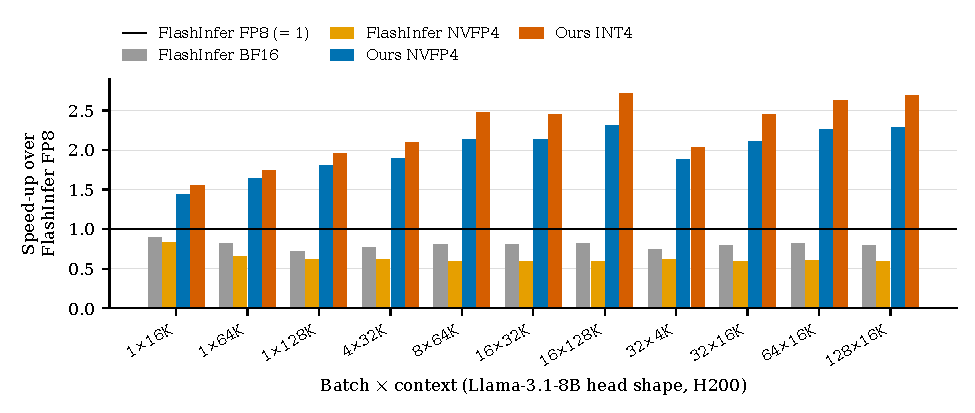
\includegraphics[width=\linewidth]{figures/fig_kernel.pdf}
\caption{Kernel speed relative to FlashInfer's FA2 FP8 kernel on H200 at all 11 shapes (one job; our times include the split merge). FlashInfer's NVFP4 is slower than its BF16 at every shape.}
\label{fig:kernel}
\end{figure}

\begin{table}[tbp]
\centering
\caption{Speed-up over FlashInfer's FA2 FP8 kernel (H200, Llama-3.1-8B head shape, one job and GPU, our times include the split merge; selected shapes). Against its XQA kernel see Table~\ref{tab:xqa}.}
\label{tab:kernel}
\small
\begin{tabular}{@{}lrrrrr@{}}
\toprule
$B \times S$ & FlashInfer FP8 (ms) & FlashInfer NVFP4 & Ours INT4 & Ours NVFP4 & Ours MXFP4 \\
\midrule
$1 \times 16$K & 0.033 & 0.83$\times$ & 1.54$\times$ & 1.43$\times$ & 1.46$\times$ \\
$1 \times 128$K & 0.116 & 0.62$\times$ & 1.95$\times$ & 1.81$\times$ & 1.83$\times$ \\
$8 \times 64$K & 0.400 & 0.59$\times$ & 2.48$\times$ & 2.14$\times$ & 2.14$\times$ \\
$32 \times 16$K & 0.395 & 0.59$\times$ & 2.44$\times$ & 2.11$\times$ & 2.11$\times$ \\
$16 \times 128$K & 1.557 & 0.59$\times$ & 2.72$\times$ & 2.31$\times$ & 2.26$\times$ \\
$128 \times 16$K & 1.542 & 0.59$\times$ & 2.70$\times$ & 2.29$\times$ & 2.27$\times$ \\
\bottomrule
\end{tabular}
\end{table}

\begin{table}[tbp]
\centering
\caption{Against FlashInfer's XQA FP8 decode kernel (H200 SXM, one job, all 11 shapes; FlashInfer 0.7.3). XQA is called as vLLM calls it (HND layout, BF16 query); the best of page sizes 16, 32, 64 and 128 is shown, with its bandwidth fraction on FP8 bytes. Ours: NVFP4, best split; the fixed split rule used inside vLLM is within 4\% of it except at $1 \times 128$K (1.79$\times$). XQA's output differs from FA2's on the same FP8 cache by at most $4.8\times10^{-3}$.}
\label{tab:xqa}
\small
\begin{tabular}{@{}lrrrrr@{}}
\toprule
$B \times S$ & FA2 FP8 (ms) & XQA FP8 (ms) & XQA bandwidth & Ours NVFP4 (ms) & Ours vs XQA \\
\midrule
$1 \times 16$K   & 0.033 & 0.027 & 26\% & 0.022 & 1.24$\times$ \\
$1 \times 64$K   & 0.070 & 0.069 & 40\% & 0.042 & 1.66$\times$ \\
$1 \times 128$K  & 0.119 & 0.121 & 46\% & 0.063 & 1.93$\times$ \\
$4 \times 32$K   & 0.118 & 0.125 & 45\% & 0.061 & 2.05$\times$ \\
$8 \times 64$K   & 0.399 & 0.343 & 65\% & 0.187 & 1.83$\times$ \\
$16 \times 32$K  & 0.402 & 0.342 & 66\% & 0.187 & 1.83$\times$ \\
$16 \times 128$K & 1.552 & 1.314 & 68\% & 0.678 & 1.94$\times$ \\
$32 \times 4$K   & 0.118 & 0.080 & 70\% & 0.061 & 1.31$\times$ \\
$32 \times 16$K  & 0.396 & 0.255 & 88\% & 0.187 & 1.37$\times$ \\
$64 \times 16$K  & 0.794 & 0.615 & 73\% & 0.352 & 1.75$\times$ \\
$128 \times 16$K & 1.552 & 0.993 & 90\% & 0.675 & 1.47$\times$ \\
\bottomrule
\end{tabular}
\end{table}

\begin{itemize}
  \item \textbf{Bandwidth.} In the job of Table~\ref{tab:kernel}, NVFP4 reaches 67\% ($B = 32$) to 75\% ($B = 128$, both at 16K) of H200's peak and INT4 74--83\%; at batch 1 it reaches far less (Section~\ref{sec:limits}). On H100 (3.35 TB/s), at batch 8 and above, NVFP4 reaches 79--86\% and INT4 82--90\%.
  \item \textbf{How much of the ratio is the baseline.} FlashInfer's FA2 FP8 kernel reaches 57\% of H200's peak at $32 \times 16$K (0.395 ms for 1.07 GB); its XQA kernel reaches 88\% there and 90\% at $128 \times 16$K, close to what a device copy achieves (86--90\%). Against XQA our margin is therefore below the byte ratio of 128/72 = 1.78$\times$ wherever XQA runs near bandwidth (1.31--1.47$\times$ at $32 \times 4$K, $32 \times 16$K and $128 \times 16$K, where we reach 51--75\%), and near or above it where XQA does not (1.75--2.05$\times$ at batch 4--64 with long contexts or many sequences, where XQA reaches 45--73\%). At batch 1, XQA gains little over FA2 at 64K and 128K, and ours is 1.24--1.93$\times$ faster. The times reported for FlashAttention-4's native FP8 on H200~\cite{fa206} imply a higher bandwidth fraction than FA2's (our arithmetic from its table, a different job), which we have not reproduced.
  \item \textbf{Where our kernel's time goes (removal ablation).} In one job on H200 SXM, with the split count fixed at the full kernel's best, we time variants that each drop one part of the work while reading the same bytes (Table~\ref{tab:ablation}). Without E2M1 reconstruction the kernel takes 0.87$\times$ the time at $B \geq 8$ (77--85\% of peak), and without the two matrix multiplies 0.92--0.94$\times$; a device copy of the same bytes reaches 87--89\%. Decoding is therefore a real but minority cost for our kernel, about 13\% of its time at $B \geq 8$; the rest of the gap to the copy ceiling is in the pipeline, the matrix multiplies and the softmax. A variant that interleaves the decoding of two rows for more instruction-level parallelism is 10--18\% slower, so we keep the simpler one. The instruction-budget diagnosis of Section~\ref{sec:stall} concerns the Triton and FlashInfer kernels, which execute two to three times the budget; ours executes about the budget in FP4 (next item), and removing its decoding saves only 13\%, so for our kernel the remaining limit is not decoding instructions alone.
  \item \textbf{FP4 on H200 is limited on the compute side, not by bytes.} MXFP4 reads 6\% fewer bytes than NVFP4 but takes the same time. An earlier build executed about 96\% of the nominal issue budget per byte, but later removing spin and address instructions gained at most 2\%, so the limit is more likely per-warp dependency chains than the issue total. On H100, with less bandwidth per instruction, both formats run near the memory limit.
  \item \textbf{With the full accuracy recipe} (K mean removal, rotation, four BF16 sinks, CUDA-graph replay), NVFP4 stays at 1.77--2.17$\times$ of FP8 for $B \geq 32$; the sink merge and q rotation add 0--7\% at $B \geq 4$, except at $16 \times 128$K (+9--13\% under CUDA graphs in two jobs, about 1\% without), and 12--31\% at $B = 1$.
  \item \textbf{Against FOSCAR} (its released code, same process and K/V, its cold-L2 timer): on H200 our INT4 is 1.08--1.61$\times$ faster at equal bytes (68 per token and head), and our NVFP4 kernel is 0.99--1.40$\times$ FOSCAR INT4's speed. With the full accuracy recipe, our NVFP4 path is slower than FOSCAR at $1 \times 16$K (1.22$\times$ vs 1.46$\times$ FlashInfer FP8), $4 \times 32$K and $32 \times 4$K (0.84--0.97$\times$ FOSCAR's speed) and faster at the other 12 shapes; this H200 run used an earlier, unfused q preparation. FOSCAR's H200 times match its published H100 numbers, so it leaves H200's extra bandwidth unused. On H100, the GPU FOSCAR was tuned for, our INT4 is 1.02--1.31$\times$ faster and our NVFP4 0.94--1.21$\times$, so the margin there is small.
\end{itemize}

\begin{table}[tbp]
\centering
\caption{Removal ablation (H200 SXM, one job, Llama-3.1-8B head shape, split count fixed at the full NVFP4 kernel's best): time relative to the full kernel (lower is faster) and fraction of peak bandwidth. Each variant drops one part of the work and reads the same bytes; ``copy'' is a device read and write of the same bytes.}
\label{tab:ablation}
\small
\begin{tabular}{@{}lrrrr@{}}
\toprule
Variant & $1 \times 64$K & $8 \times 64$K & $32 \times 16$K & $128 \times 16$K \\
\midrule
Full NVFP4 kernel (ms)            & 0.042 & 0.188 & 0.188 & 0.675 \\
No E2M1 reconstruction            & 0.98 & 0.87 & 0.87 & 0.87 \\
No matrix multiplies              & 0.97 & 0.92 & 0.92 & 0.94 \\
Interleaved decoding (ILP)        & 1.08 & 1.10 & 1.11 & 1.18 \\
MXFP4                             & 0.98 & 1.01 & 0.99 & 1.01 \\
INT4                              & 0.93 & 0.87 & 0.87 & 0.85 \\
\midrule
Full kernel, fraction of peak     & 38\% & 67\% & 67\% & 75\% \\
No reconstruction, fraction of peak & 39\% & 77\% & 77\% & 85\% \\
Copy of the same bytes            & 76\% & 87\% & 87\% & 89\% \\
\bottomrule
\end{tabular}
\end{table}

How the instruction count came down: the first K-side prototype reached 60\% of bandwidth at 3.0 instructions per value. NVBit then showed three compiler-level wastes (a LOP3 split into two instructions, wgmma descriptors recomputed per instruction, idle lanes doing softmax work); fixing them gave 1.95 instructions per value and 72\% (87\% in steady state).

\section{End-to-end in vLLM}
\label{sec:e2e}

Inside vLLM 0.33.0, with the full recipe used for every accuracy number in Section~\ref{sec:accuracy}, our plugin decodes 1.12--1.64$\times$ faster than FlashInfer FP8 (XQA decode) at batch 8 and above, and is level with it at batch 1 (1.01--1.05$\times$ per decode step, 0.96--1.03$\times$ in end-to-end time per output token). vLLM's own NVFP4 KV path is 1.4--2.3$\times$ slower than FP8 at batch 8 and above. Our cache holds 1.63$\times$ as many tokens, and time to first token is 1.5--6\% slower. Under a reasoning-like request stream both meet latency targets up to 1.25 requests/s on Llama-3.1-8B, ours with lower time per output token; above that FP8's cache fills first. The highest rate one H200 sustains is 1.23--1.32$\times$ FP8's on Llama-3.1-8B, 1.45--1.80$\times$ on Qwen3-32B and 1.67--2.20$\times$ on Qwen2.5-72B (Table~\ref{tab:capacity}).

The plugin replaces the cache write, decode and prefill attention of vLLM's 4-bit backend with our kernels, and runs prefill attention on FlashAttention-3 in BF16. Pure decode time per step is in Table~\ref{tab:e2e} and Figure~\ref{fig:vllm}.

\begin{table}[tbp]
\centering
\caption{Pure decode time per step (\texttt{vllm bench forward}, Llama-3.1-8B, H200 SXM, all configurations in one job; median of 100 CUDA-graph replays). FP8: FlashInfer with XQA decode (resolved kernel logged); vLLM NVFP4: \texttt{-{}-kv-cache-dtype nvfp4}, FlashInfer's native decode; ours: the full recipe, every sequence on the sink path. Speed-ups are over FP8.}
\label{tab:e2e}
\small
\begin{tabular}{@{}lrrrrr@{}}
\toprule
$B \times$ context & FP8 (ms) & vLLM NVFP4 (ms) & Ours (ms) & vLLM NVFP4 & Ours \\
\midrule
$1 \times 16$K   & 4.97  & 5.52  & 4.92  & 0.90$\times$ & 1.01$\times$ \\
$1 \times 32$K   & 5.57  & 6.42  & 5.31  & 0.87$\times$ & 1.05$\times$ \\
$8 \times 16$K   & 7.50  & 10.43 & 6.69  & 0.72$\times$ & 1.12$\times$ \\
$8 \times 32$K   & 10.25 & 15.69 & 8.06  & 0.65$\times$ & 1.27$\times$ \\
$32 \times 16$K  & 12.66 & 26.36 & 10.94 & 0.48$\times$ & 1.16$\times$ \\
$32 \times 32$K  & 20.42 & 47.80 & 16.43 & 0.43$\times$ & 1.24$\times$ \\
$64 \times 16$K  & 24.80 & 48.23 & 16.74 & 0.51$\times$ & 1.48$\times$ \\
$16 \times 64$K  & 26.90 & 47.59 & 16.35 & 0.57$\times$ & 1.64$\times$ \\
$128 \times 8$K  & 21.81 & 49.18 & 17.43 & 0.44$\times$ & 1.25$\times$ \\
\bottomrule
\end{tabular}
\end{table}

\begin{figure}[tbp]
\centering
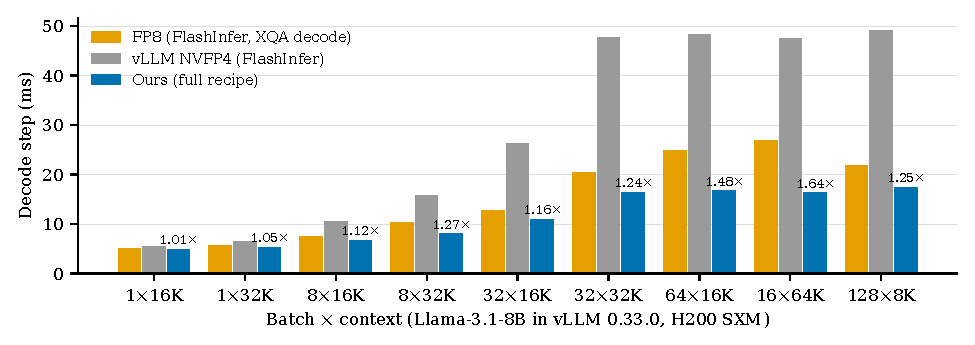
\includegraphics[width=\linewidth]{figures/fig_vllm.pdf}
\caption{Decode step time in vLLM (data of Table~\ref{tab:e2e}); labels give the speed-up.}
\label{fig:vllm}
\end{figure}

Mean removal and sinks cost 1.2--3.2\% against NVFP4 with only layer 0 in BF16 (both in one earlier job on an H200 SXM node; the table's job does not include that configuration). On two other models (one job each, H200 SXM, contexts up to 32K): Qwen3-32B 1.00--1.02$\times$ at batch 1 and 1.05--1.18$\times$ at batch 8 and above; Qwen3-30B-A3B (MoE) 0.94--0.95$\times$ at batch 1 and 1.11--1.32$\times$ at batch 8 and above. On UltraQuant's own format (MXFP4 with K rotation, the same bytes per token, vLLM's default four BF16 boundary layers; one job, H200 SXM, the shapes of Table~\ref{tab:e2e}), our kernel decodes 1.9--5.1$\times$ faster per step than vLLM's stock UltraQuant backend, which falls back to Triton on NVIDIA, and is 1.03--1.06$\times$ FlashInfer FP8 at batch 1 and 1.08--1.48$\times$ at batch 8 and above; the stock backend is 1.8--3.9$\times$ slower than FP8.

End to end (\texttt{vllm bench latency}, full recipe vs FlashInfer FP8, two consecutive jobs on one H200 SXM node): time per output token 5.30 vs 5.08 ms at $1 \times 16$K (0.96$\times$), 5.55 vs 5.72 at $1 \times 32$K (1.03$\times$), 6.95 vs 7.77 at $8 \times 16$K (1.12$\times$), 8.60 vs 10.94 at $8 \times 32$K (1.27$\times$) and 12.77 vs 13.94 at $32 \times 16$K (1.09$\times$). Offline throughput (8K and 16K input, 512 output tokens, 256 requests) is 1.06--1.10$\times$ in the same jobs. The KV cache holds 2,867,200 tokens against 1,761,600 for FP8 at the same memory setting (1.63$\times$). Decode-led throughput (16K in, 2,048 out, 256 requests) is 1.17$\times$ against FlashInfer FP8 and 1.40$\times$ against the default FlashAttention-3 FP8 path; these three runs are separate jobs on H200 SXM, and the FP8 runs predate a plugin change that does not affect them. At $64 \times 32$K (both configurations in one job, H200 SXM), where FP8's cache cannot hold all 64 sequences (2.1M tokens against 1.76M) and ours can, decode time per output token is 38.7 vs 52.2 ms (1.35$\times$); the whole request with 256 output tokens still takes 86.8 vs 85.0 s (2\% longer), because prefill of the 2.1M prompt tokens is 7\% slower (77.0 vs 71.7 s).

\begin{itemize}
  \item \textbf{Why the gain is smaller than the kernel's 2$\times$.} Each step also reads the 16 GB of BF16 weights, at least 3.3 ms at H200's peak bandwidth, against 6.69 ms for our whole step at $8 \times 16$K; attention is a minority of the step, and the gain grows with context and batch. A per-kernel profile at $8 \times 16$K (both configurations in one job, H200 SXM, 32 decode steps) shows the split: our decode kernel takes 1.50 ms per step against FlashInfer's 2.88 ms (1.92$\times$), and with the sink merge, the cache write, the q rotation and layer 0 in BF16, the attention-related kernels total 2.00 against 3.02 ms, about a quarter of our step (7.55 vs 8.43 ms under the profiler); the GEMMs take about 4.0 ms in both.
  \item \textbf{Why FlashInfer FP8 is the baseline.} vLLM's default FP8 path (FlashAttention-3 with an FP8 query) was slower than FlashInfer at large batch in our runs ($32 \times 32$K on H200 NVL: 30.2 vs 21.6 ms per step, same job), so all ratios above are against FlashInfer; against the default they are larger (decode-led throughput 1.40$\times$ vs 1.17$\times$). FlashInfer's FP8 decode inside vLLM is the XQA kernel: forcing it with \texttt{VLLM\_HAS\_FLASHINFER\_CUBIN=1} changes the step time by at most 0.3\% (same job as Table~\ref{tab:e2e}).
  \item \textbf{Prefill.} vLLM's 4-bit backends run prefill attention on FlashAttention-2; we switch to FlashAttention-3 in BF16 (also proposed in vLLM PR \#47531). Prefill alone is still 7\% slower than FlashInfer FP8 (8 prompts of 32,000 tokens: 9.29 vs 8.66 s, same job), and time to first token is 1.5--6\% slower end to end. About a third of the gap is prefill attention: FlashInfer's FP8 prefill attention is about 226 ms faster than our BF16 one. An FP8 prefill path could close that part, at an accuracy cost we measured only on an earlier all-layer MXFP4 configuration (perplexity +1.51\% vs +0.68\% with BF16 prefill, Llama-3.1-8B, H200 NVL). Most of the rest is copies and small ops ($\sim$230 ms) and dequantization for continued prefill (72 ms). With prefill and decode on separate GPUs, the decode pool does not run prefill.
\end{itemize}

\paragraph{Serving under load.} We ran \texttt{vllm serve} with Poisson arrivals at fixed request rates (Llama-3.1-8B, H200 SXM; random prompts with input and output lengths uniform within $\pm$50\% of the nominal values; arrivals for 600 s, or 300 s for the 16K-input workload; both configurations one after the other in the same job, FP8 with XQA decode). A request meets the service-level objective (SLO) if its time to first token is at most 2 s and its time per output token at most 100 ms (the MLPerf Llama-3.1-8B server targets); a rate is sustainable if at least 99\% of requests meet it. Intervals resample requests (1000 draws) and so do not include run-to-run variation; Table~\ref{tab:serve} lists the runs.

\begin{table}[tbp]
\centering
\caption{Serving under load (Llama-3.1-8B, H200 SXM, FP8 with XQA decode). Share of requests meeting the SLO [95\% request-bootstrap interval], peak KV-cache use, and FP8's preemptions (ours: none in the reasoning-like runs listed; 13 in the long-context run at 1.5). One vLLM API-server process (the default) and seed 0 unless noted. At 1.25, comma-separated values are seed 0 and seed 1 for both. At 1.35 and 1.5, comma-separated values are separate runs: FP8 seed 0 and seed 1; ours seed 0, a repeat of seed 0 with the same arrivals (on the same node at 1.35, another H200 SXM node at 1.5) and seed 1. ``4 API'': seeds 0 and 1 with \texttt{-{}-api-server-count 4}. Mean TPOT is time per output token.}
\label{tab:serve}
\small\setlength{\tabcolsep}{2.5pt}
\begin{tabular}{@{}lrlrlrl@{}}
\toprule
Workload & Rate & FP8: SLO share & KV & Ours: SLO share & KV & Notes \\
\midrule
Reasoning-like  & 0.75 & 1.00 & 32\% & 1.00 & 16\% & mean TPOT 13.3 vs 10.3 ms \\
(1K in, 8K out) & 1.0  & 1.00 & 59\% & 1.00 & 29\% & mean TPOT 19.5 vs 14.3 ms \\
                & 1.25 & 1.00, 1.00 & 93--97\% & 1.00, 1.00 & 46\% & mean TPOT 28.2 vs 20.6 ms \\
                & 1.35 & 0.89, 0.94 & 100\% & 0.82, 1.00, 0.86 & 55--59\% & FP8: 628, 656 preemptions \\
                &      & 0.88, 0.94 & 100\% & 1.00, 1.00 & 58--61\% & 4 API; FP8: 683, 651 \\
                & 1.4  & 0.82 [0.80, 0.85] & 100\% & 1.00 & 62\% & FP8: 750 preemptions \\
                & 1.5  & 0.69, 0.75 & 100\% & 0.81, 1.00, 1.00 & 78--79\% & FP8: 1513, 1375 preemptions \\
                &      & 0.69, 0.75 & 100\% & 1.00, 1.00 & 79--81\% & 4 API; FP8: 1494, 1374 \\
\midrule
Long context    & 0.5  & 0.99 & 19\% & 0.99 & 11\% & \\
(16K in, 1K out) & 1.0 & 0.87 [0.83, 0.90] & 66\% & 0.84 [0.80, 0.88] & 35\% & \\
                & 1.5  & 0.14 [0.11, 0.18] & 100\% & 0.04 [0.03, 0.06] & 100\% & both prefill-bound \\
\midrule
Prefill-heavy   & 0.75 & 0.98 [0.96, 1.00] & 19\% & 0.94 [0.90, 0.97] & 12\% & p99 TTFT 2.2 vs 2.5 s \\
(16K in, 512 out) & 1.25 & 0.87 [0.83, 0.90] & 57\% & 0.77 [0.73, 0.82] & 37\% & p99 TTFT 4.0 vs 4.4 s \\
\bottomrule
\end{tabular}
\end{table}

\begin{itemize}
  \item \textbf{Reasoning-like} (1K input, 8K output). Up to 1.25 requests/s both meet the SLO for every request in these runs, and also with four API-server processes at 0.25 and 0.5 and, with seed 2, at 1.25 (where FP8's cache is full, with 190 preemptions); ours has 23--27\% lower mean time per output token, 12\% more output tokens per second at 1.25, and half the KV-cache use (FP8 is at 97\% at 1.25). From 1.35 on, FP8's cache is full in every run: requests wait and are preempted (628--1513 preemptions), and 6--31\% miss the time-to-first-token target. Our cache never exceeds 81\%, and at 1.4 every request meets the SLO (goodput 1.01 against 0.71 requests/s).
  \item \textbf{Our misses near saturation come from vLLM's API server, not from the cache.} With one API-server process, vLLM's default, ours met the SLO for 82\%, 100\% and 86\% of requests in three runs at 1.35, and for 81\%, 100\% and 100\% at 1.5. Every miss was a first-token delay of 2--6 s while no request was waiting in vLLM's scheduler and none was preempted, and the client sent every request on schedule. In the seed-1 run at 1.35, the API-server process used 92--97\% of one CPU core for about eight minutes (our server streams about 8,200 output tokens per second), and vLLM's own metrics place the delay in that process: 92 of the 814 requests the server counted (including the benchmark's 5 warm-up requests) had a time to first token above 2.5 s as the server measured it, while the scheduler's queue time summed to 0.009 s over all 814 and prefill took 69 ms on average. With four API-server processes (\texttt{-{}-api-server-count 4}, seeds 0 and 1), ours met the SLO for every request at both rates in both seeds (p99 time to first token at most 0.16 s at 1.35 and 0.69 s at 1.5), and FP8 did not change (0.88 and 0.94 at 1.35, 0.69 and 0.75 at 1.5, against 0.89--0.94 and 0.69--0.75 with one process; 651--1494 preemptions): its misses come with a full cache in every run. So at these rates a single API-server process limits vLLM before our cache does, and FP8's cache limits it before that.
  \item \textbf{Two runs of ours that did not reproduce.} Both stay in the result files. (i) Seed 2 at 1.25 and 1.5 requests/s with one API-server process met the SLO for 5\% and 3\% of requests: time per output token was already 114 ms at the first request, at almost no load (7--9 ms on average at 0.25--0.5 requests/s in the other runs), the cache filled and 1002 and 1202 requests were preempted, while seed 1 ran normally on another GPU of the same node at the same time. A rerun of seed 2 at 1.25 (four API-server processes, another node) met the SLO for every request (7,986 output tokens per second, cache peak 46\%). (ii) Seed 0 at 0.25 and 0.5 requests/s with one API-server process met it for 97\% and 87\%, all misses being first-token delays of 2--3 s at 5--10\% cache use, spread over the run; a rerun with the same settings and one with four API-server processes met it for every request.
  \item \textbf{Long context} (16K input, 1K output). Both are sustainable at 0.5 requests/s and level at 1.0 (0.87 vs 0.84, intervals overlapping), although ours uses half the cache. At 1.5, 24K prompt tokens arrive per second, close to what either server can prefill (Section~\ref{sec:e2e}, prefill), both caches fill with partly prefilled requests, and both fail; ours fails more (0.04 vs 0.14, p99 time per output token 149 vs 94 ms), consistent with its 7\% slower prefill. A larger cache does not help a prefill-bound stream.
  \item \textbf{Prefill-heavy} (16K input, 512 output). FP8 keeps more requests within the SLO at both rates we ran: 0.98 vs 0.94 at 0.75 requests/s and 0.87 vs 0.77 at 1.25 (intervals not overlapping at 1.25), with neither cache near full and no preemptions. The 99th-percentile time per output token stays under the 100 ms target for both (89 vs 94 ms at 1.25), so almost all misses are first-token delays, consistent with our 7\% slower prefill; with short outputs there is no decode advantage to offset it. Ours alone at 0.5, 1.0 and 1.5 requests/s: 0.85, 0.65, 0.16 (no FP8 run at those rates).
\end{itemize}

\paragraph{Capacity on one GPU, from 8B to 72B.} For serving cost, the number that matters is the highest request rate one GPU sustains. Table~\ref{tab:capacity} gives it for three models under the reasoning-like stream, with each bracket refined to a width of at most 0.05 requests/s. The gain grows with model size, from 1.23--1.32$\times$ on Llama-3.1-8B to 1.45--1.80$\times$ on Qwen3-32B and 1.67--2.20$\times$ on Qwen2.5-72B, while the per-step gain shrinks from 1.12--1.64$\times$ (1.15--1.70$\times$ with FP8 weights) to 1.04--1.18$\times$: a larger model's step is dominated by its weight read (about 71 GB per step for the 72B model), and its weights leave less memory for the cache, consistent with the cache, rather than its bandwidth, setting the limit. On the two larger models FP8's cache is almost full at its highest sustainable rate in seed 0 (99.9\% on Qwen3-32B at 0.25, 95\% on Qwen2.5-72B at 0.125 requests/s; the seed-1 repeats peaked at 68\%), and at the next rate requests are preempted and miss the time-to-first-token target. Our own highest sustainable rate on Qwen2.5-72B is close to its cache limit too: at 0.25 requests/s in seed 0 the cache filled, 57 requests were preempted and 149 of 150 met the SLO (seed 1: 80\% peak, none preempted). On Llama-3.1-8B the gain stays below the 1.63$\times$ token ratio: at its first failing rate (1.65) our cache is 96\% full with no preemptions, and we did not isolate what limits it there. On Qwen2.5-72B the gain is at least the 1.61$\times$ token ratio; we did not isolate how much FP8's preemptions (94 at 0.15 requests/s) add to it. On the 72B model ours is also the more accurate configuration: in vLLM, wikitext-2 perplexity ($16 \times 8192$ tokens, FP8 weights) is 0.95\% above BF16 KV for FP8 (0.88\% with layer 0 in BF16) and 0.03\% for ours.

\begin{table}[tbp]
\centering
\caption{Single-GPU capacity (\texttt{results/serve\_goodput\_x\_11-21.csv}; reasoning-like workload: 1K input, 8K output, lengths uniform within $\pm$50\%; Poisson arrivals, $\max(150, 600\,\mathrm{s} \times \mathrm{rate})$ requests; H200 SXM; four API-server processes; FP8 with XQA decode). The highest sustainable rate is the highest rate at which at least 99\% of requests meet the SLO (time to first token $\leq$ 2 s, time per output token $\leq$ 100 ms): [highest rate that held, lowest rate that failed), seed 0; the boundary points marked $^{\dagger}$ were repeated with seed 1, and Llama-3.1-8B's FP8 point at 1.25 also holds with seed 2. KV tokens: vLLM's reported cache size at \texttt{-{}-gpu-memory-utilization 0.9} in these serving runs (\texttt{-{}-max-model-len 14336}, \texttt{-{}-max-num-seqs 512}); the latency and throughput runs of Section~\ref{sec:e2e} use other engine settings and report 2.87M and 1.76M on Llama-3.1-8B, the same 1.63$\times$ ratio. Per step: pure decode speed-up over FP8 at batch 8 and above (\texttt{vllm bench forward}; Llama-3.1-8B and Qwen3-32B with BF16 weights, Qwen2.5-72B with FP8 weights, its shapes up to $32 \times 8$K and $8 \times 31$K). The SLO targets are the same for all three models. Qwen2.5-72B-Instruct uses FP8 weights (RedHatAI FP8-dynamic) to fit on one GPU.}
\label{tab:capacity}
\small\setlength{\tabcolsep}{3pt}
\begin{tabular}{@{}lrrllrr@{}}
\toprule
 & \multicolumn{2}{c}{KV tokens} & \multicolumn{2}{c}{Highest sustainable rate (req/s)} & & Per step \\
\cmidrule(lr){2-3}\cmidrule(lr){4-5}
Model & FP8 & Ours & FP8 & Ours & Ratio & $B \geq 8$ \\
\midrule
Llama-3.1-8B          & 1.78M & 2.90M & [1.25, 1.3)  & [1.6, 1.65)$^{\dagger}$  & 1.23--1.32$\times$ & 1.12--1.64$\times$ \\
Qwen3-32B             & 0.50M & 0.82M & [0.25, 0.275)$^{\dagger}$ & [0.4, 0.45)$^{\dagger}$  & 1.45--1.80$\times$ & 1.05--1.18$\times$ \\
Qwen2.5-72B (FP8 w.)  & 0.34M & 0.54M & [0.125, 0.15)$^{\dagger}$ & [0.25, 0.275)$^{\dagger}$ & 1.67--2.20$\times$ & 1.04--1.18$\times$ \\
\bottomrule
\end{tabular}
\end{table}


\section{Accuracy}
\label{sec:accuracy}

Inside vLLM, the full recipe shows no difference from BF16 KV larger than run-to-run noise on any model or task we tested, from 7B to 32B and on an MoE model; five models have repeated runs with a paired test, and three rows are single runs. Offline, it stays within our preset bound (perplexity +0.1, KL 0.02) on Llama-3.1-8B, Mistral-7B and Qwen3-8B-Base. Without layer-0 protection, Qwen2-family reasoning models collapse, even under FP8.

\providecommand{\pend}{\textcolor{gray}{pend.}}
\begin{table}[tbp]
\centering
\caption{What each KV-cache option gives on H200 (Llama-3.1-8B for speed, perplexity and KL). Bytes per 128-value
row of K or V, scales included. Speed: \texttt{vllm bench forward} decode step, all rows in one job, as a speed-up
over vLLM's FlashInfer FP8 path (XQA decode; higher is faster). MATH-500 (Qwen2.5-7B-Instruct, R1-Distill-Llama-8B, Phi-4) inside vLLM, mean over runs; perplexity increase over BF16 inside vLLM
(wikitext-2, $16\times8192$; Qwen2.5-7B-Instruct and Llama-3.1-8B); KL offline (FP32, $8\times2048$). One scale per tensor has no decode kernel in vLLM or
FlashInfer, so it has only offline numbers. KL: no sinks except ours (four); ours with the window K mean. vLLM NVFP4 is \texttt{-{}-kv-cache-dtype nvfp4} with vLLM's defaults
(every layer, global scale 1.0); $\times$246: perplexity 1542 against 6.27 (FP8: 231). MATH-500 of vLLM NVFP4: three runs each; FP8: one run each. $^*$BF16 at the three shapes whose cache fits (8$\times$16K, 8$\times$32K, 32$\times$16K tokens; at 64$\times$16K and above it does not), from a second job that reran FP8 and ours (ours there 1.12--1.63$\times$).}
\label{tab:baselines}
\small\setlength{\tabcolsep}{2.9pt}
\begin{tabular}{@{}lrrrrrrrrr@{}}
\toprule
& & \multicolumn{2}{c}{Speed-up vs FP8} & \multicolumn{3}{c}{MATH-500 (\%)} & \multicolumn{2}{c}{$\Delta$ppl} & Llama \\
\cmidrule(lr){3-4}\cmidrule(lr){5-7}\cmidrule(lr){8-9}
KV cache & Bytes & $B\geq8$ & $B=1$ & Qwen2.5 & R1-Llama & Phi-4 & Qwen2.5 & Llama & KL \\
\midrule
BF16                                & 256 & 0.63--0.86$^*$ & 0.96--0.97 & 71.2 & 67.7 & 75.3 & -- & -- & -- \\
FP8 (FlashInfer XQA)                & 128 & 1.00  & 1.00  & 1.6 & 67.0 & 76.0 & $\times$36.8 & +0.94\% & 0.0037 \\
4-bit, one scale/tensor & 64 & -- & -- & -- & -- & -- & -- & -- & 0.297 \\
vLLM NVFP4                          & 72  & 0.43--0.72 & 0.87--0.90 & 0.0 & 68.4 & 74.9 & $\times$246 & +2.62\% & 0.0282 \\
\quad layer 0 in BF16            & 72  & --    & --    & 65.9 & --    & --    & +78\% & +2.56\% & 0.0262 \\
Ours (full recipe)                  & 72  & 1.12--1.64 & 1.01--1.05 & 72.0 & 67.7 & 74.1 & +0.05\% & +0.06\% & 0.0103 \\
\bottomrule
\end{tabular}
\end{table}

\begin{table}[tbp]
\centering
\caption{Each step of the recipe, added one at a time: mean KL against BF16 (offline, FP32, wikitext-2,
$8\times2048$ tokens, the K mean taken over each window; (a)--(c) without sinks, (d)--(f) and FP8 as noted in the text). None of the steps is ours; the table measures what each
contributes on one setup.}
\label{tab:ladder}
\small
\begin{tabular}{@{}llrrr@{}}
\toprule
& Step & Llama-3.1-8B & Qwen2.5-7B-I & Qwen3-8B-Base \\
\midrule
(a) & 4-bit FP4, one scale per tensor           & 0.297  & 10.1  & 3.00 \\
(b) & NVFP4: an E4M3 scale per 16 values        & 0.0269 & 5.90  & 0.0291 \\
(c) & + Hadamard rotation of K~\cite{ashkboos2024quarot} & 0.0187 & 6.95 & 0.281 \\
(d) & + 4 BF16 sink tokens~\cite{xiao2023streamingllm,liu2024intactkv} & 0.0168 & 7.05 & 0.249 \\
(e) & + K mean removal~\cite{zhang2025sageattention,shao2026flagrot}  & 0.0111 & 0.0167 & 0.0125 \\
(f) & + layer 0 in BF16                         & 0.0103 & 0.0147 & 0.0097 \\
\midrule
    & FP8, one scale per tensor (reference)     & 0.0037 & 3.86  & 0.0040 \\
\bottomrule
\end{tabular}
\end{table}

\paragraph{What each step fixes.}
Steps (a)--(c) run without sinks, (d)--(f) with four; FP8 is as vLLM ships it (every layer, no sinks).
\textbf{(a)$\to$(b) Block scales.} With one scale per tensor, the largest value in the layer sets the step size;
E2M1's smallest non-zero value is $0.5$ of that scale, so where K has a channel or token tens of times larger than
the typical value, most entries round to zero. A scale per 16 values confines an outlier to its own block: KL falls
11$\times$ on Llama and 103$\times$ on Qwen3-8B-Base. (INT4 with one scale per tensor is worse still: 1.74 and 4.26.)
Fixing NVFP4's global scale at 1.0, as vLLM stores it, changes the KL by at most 1.3\% on these two models.
\textbf{(b)$\to$(c) Rotation.} Within a block an outlier channel still sets the scale for the other 15 values; a
Hadamard rotation spreads each channel over all 128, and lowers Llama's KL by 30\%. On Qwen3-8B-Base it does the
opposite (0.029 to 0.281): K there has a large per-channel mean, and the rotation spreads it into every block,
where it takes over the scale (KV4-RL~\cite{park2026kv4rl}, Appendix D.4, also finds that K rotation raises NVFP4 KV mismatch on Qwen3 models without mean removal). Once the mean is removed (four sinks, layer 0 in BF16, one job per model), rotation
still lowers the KL, but only by 12\% on Llama, 14\% on Qwen2.5-7B-Instruct and 8\% on Qwen3-8B-Base.
\textbf{(c)$\to$(d) Sinks.} The first tokens receive a large share of the attention mass in most layers, so their
error weighs more than other tokens'. Before the mean is removed, sinks help little (Llama $-10\%$). With the mean
removed (recipe without the static mean, sink 0, 1, 2, 4, 8, 16), one sink already gives 98\% of the gain of four on
Llama, 101\% on Qwen3-8B-Base and 80\% on Qwen2.5-7B-Instruct (two give 97\%), and 8 or 16 add nothing we can
resolve: the gain is the first token, and four leave a margin.
\textbf{(d)$\to$(e) Mean removal.} The per-channel K mean is shared by all tokens and cancels in the softmax
($q\cdot\mu$ is the same for every key), so subtracting it before quantizing removes energy the scales would
otherwise spend on it, at no read-time cost. It is the step that rescues the Qwen models: Qwen2.5-7B-Instruct
goes from 7.05 (collapsed, as FP8 is at 3.86) to 0.0167, Qwen3-8B-Base from 0.249 to 0.0125, both close to Llama's
0.0111. It needs the sinks: at sink 0 it makes Llama worse, not better (0.0233 against 0.0187).
\textbf{(e)$\to$(f) Layer 0.} In Qwen2-family models the key-projection bias makes layer 0's K almost entirely its
mean (98\% of the norm on R1-Distill-Qwen-7B); keeping that layer in BF16, at 1/28--1/32 of the cache, lowers the
KL by a further 12\% on Qwen2.5-7B-Instruct, 22\% on Qwen3-8B-Base and 7\% on Llama (one job each).
On its own it is not enough for 4-bit: on Qwen2.5-7B-Instruct, NVFP4 with four sinks and only layer 0 in BF16 has a
KL of 0.250, 17$\times$ the recipe's 0.0146, while the same protection takes FP8 from 3.79 to 0.033 (one job, four BF16 sinks in every configuration; Table~\ref{tab:ladder}, from other jobs, gives 0.0147 for the recipe and 3.86 for FP8 without sinks).
Inside vLLM the order is the same (Table~\ref{tab:baselines}): on Llama-3.1-8B, perplexity rises by 2.62\% with vLLM's NVFP4, 2.56\% with its layer 0 in BF16, 0.94\% with FP8 and 0.06\% with the recipe; on Qwen2.5-7B-Instruct, vLLM's NVFP4 with only layer 0 in BF16 still raises perplexity by 78\% and scores 65.9\% on MATH-500 against BF16's 71.2\% ($-$5.3 points, 95\% CI [$-$8.4, $-$2.4], $p < 0.001$, three runs against five), while the recipe scores 72.0\%.
\textbf{vLLM's NVFP4 as shipped} corresponds to (b) with the global scale fixed at 1.0 and no layer protection:
offline it is (b) within 1.3\% on Llama and Qwen3 in one job (the 0.0282 of Table~\ref{tab:baselines} comes from another job, which measured both vLLM NVFP4 rows; separate jobs differ by up to 4\%) and collapsed on Qwen2.5-7B-Instruct (4.91).
Inside vLLM it is accurate on the two models without a key bias, R1-Distill-Llama-8B ($+0.7$ points against BF16, 95\% CI [$-$2.4, +3.9], $p = 0.60$) and Phi-4 ($-$0.3, [$-$2.6, +1.9], $p = 0.80$; three runs each), and collapses on Qwen2.5-7B-Instruct (0.0\% on MATH-500 in all three runs, perplexity 1542 against 6.27), as FP8 does (1.6\%). Away from the Qwen2 family its cost is speed: it decodes 1.4--2.3$\times$ slower than FP8 at batch 8 and above (Table~\ref{tab:e2e}).
\textbf{Context length.} On Llama with four sinks, the recipe's KL (window mean, layer 0 in BF16) moves from
0.0093 at 2K tokens to 0.0113 at 16K, and its ratio to FP8 from 3.0 to 2.7 (32K tokens per point).



\paragraph{Offline perplexity and KL} (simulated quantization after RoPE, wikitext-2~\cite{merity2016pointer}, $16 \times 4096$ tokens, first 4 tokens in BF16; Table~\ref{tab:offline}).

\begin{table}[tbp]
\centering
\caption{Offline KL against BF16 and perplexity increase (in parentheses); simulated quantization after RoPE, wikitext-2, $16 \times 4096$ tokens, first 4 tokens in BF16. The K mean here is taken over each window; a mean from the first 512 tokens is 8--14\% worse, and inside vLLM the mean is a static calibration.}
\label{tab:offline}
\begin{tabular}{@{}llll@{}}
\toprule
Model & NVFP4, K rotated & NVFP4, K mean-removed + rotated & FP8 \\
\midrule
Llama-3.1-8B & KL 0.0165 (+0.097) & KL 0.0115 (+0.065) & +0.015 \\
Mistral-7B-v0.3 & KL 0.0071 (+0.030) & KL 0.0060 (+0.025) & +0.007 \\
Qwen3-8B-Base & KL 0.210 (+1.38) & KL 0.0114 (+0.041) & $\leq$ +0.015 \\
\bottomrule
\end{tabular}
\end{table}

Rotation lowers each 4-bit format's error 1.6--2.9$\times$ on Llama and Mistral with sinks (up to 3.3$\times$ without); the order is NVFP4, then INT4, then MXFP4. On Qwen3, rotation alone raises NVFP4's KL to 0.210, 18 times that of the mean-removed version: the per-channel mean of K, shared by all tokens, holds about half of K's energy and in some Qwen3 layers sits in one channel, and rotation spreads it into every 16-value group (FlagRot reports the same harm for whole-head rotation on Qwen3-8B). Removing the mean first (SageAttention's smooth K, also part of BitDecoding-FP4's recipe) fixes it at no read-time cost, since $q \cdot \mu$ is the same for every token. Mean removal needs the sink: without it, Llama is 25\% worse. These KL values were computed in BF16; recomputing Llama-3.1-8B's in FP32 lowers FP8's KL by 17--18\% and the 4-bit formats' by 2--6\%, and leaves the order of formats unchanged.

\paragraph{Inside vLLM} (vLLM 0.33.0, full recipe against BF16 KV; Table~\ref{tab:invllm}). Greedy decoding in vLLM is not reproducible across runs, because batch composition changes the numerics: on R1-Distill-Llama-8B, three BF16 runs score 68.4\%, 67.0\% and 67.6\% on MATH-500~\cite{hendrycks2021math,lightman2023verify}, and any two of them disagree on about 47 of 500 problems. So the reasoning rows use several runs with shuffled submission order, and a paired permutation test on each problem's mean correctness; a single-run difference within $\pm$3 points is not evidence either way. Runs used both H200 variants; within a row, BF16 and ours ran on the same variant, except one of the three R1-Distill-Llama-8B run pairs.

\begin{table}[tbp]
\centering
\caption{Inside vLLM (vLLM 0.33.0, H200, full recipe against BF16 KV). For single runs no $p$ is given: a single-run test assumes fixed per-problem outcomes, which the run-to-run variation above contradicts. Intervals: two-level bootstrap (problems, then runs within each configuration, 2000 draws); $^{*}$one run, so the interval resamples problems only and omits run-to-run variation.}
\label{tab:invllm}
\small
\begin{tabularx}{\linewidth}{@{}P{4.2cm}LP{1.5cm}rrl@{}}
\toprule
Model & Test & Runs & BF16 & Ours & Ours $-$ BF16 [95\% CI] ($p$) \\
\midrule
Qwen2.5-7B-Instruct & MATH-500 & 5 & 71.2 & 72.0 & +0.8 [$-$1.6, +3.3] (0.49) \\
DeepSeek-R1-Distill-Qwen-7B & MATH-500 & 5 & 70.8 & 71.2 & +0.4 [$-$2.0, +3.1] (0.71) \\
DeepSeek-R1-Distill-Llama-8B & MATH-500 & 3 & 67.7 & 67.7 & +0.07 [$-$3.1, +3.3] (1.0) \\
Phi-4 & MATH-500 & 3 & 75.3 & 74.1 & $-$1.2 [$-$3.5, +1.1] (0.33) \\
Qwen3-32B, thinking on & MATH-500, first 200, 16K tokens & 3 & 90.0 & 90.3 & +0.3 [$-$2.7, +3.2] (0.89) \\
Qwen3-32B, thinking off & MATH-500 & 1 & 78.6 & 79.2 & +0.6 [$-$1.6, +2.8]$^{*}$ (--) \\
Qwen3-30B-A3B (MoE), thinking off & MATH-500 & 1 & 79.2 & 79.0 & $-$0.2 [$-$2.6, +2.2]$^{*}$ (--) \\
Llama-3-8B-ProLong-512k-Instruct & RULER-style~\cite{hsieh2024ruler} multi-key / multi-value / variable tracking, 32K--120K & 1 (450 paired trials) & -- & -- & +0.6 points (0.50) \\
\bottomrule
\end{tabularx}
\end{table}

MATH-500 rows use all 500 problems unless noted. Qwen2.5-7B and R1-Distill-Qwen-7B have $G = 7$ and ran through our kernel with q zero-padded to 8 heads. Perplexity in vLLM (wikitext-2, $16 \times 8192$ tokens; OLMo-2 $16 \times 4000$), increase over BF16, ours vs FP8: Llama-3.1-8B +0.06\% vs +0.94\%; Qwen3-32B +0.07\% vs +0.59\%; Phi-4 +0.15\% vs +0.30\%; OLMo-2-1124-7B +0.06\% vs +0.34\%; Qwen3-30B-A3B +0.07\% vs +0.04\%; Qwen2.5-72B-Instruct with FP8 weights +0.03\% vs +0.95\%. Within the recipe, mean removal and sinks matter: on Qwen2.5-7B-Instruct, NVFP4 with only layer 0 in BF16 scores 69.3\% over 5 runs, 2.7 points below the full recipe ($p = 0.035$).

\paragraph{Long context, offline.} On LongBench~\cite{bai2024longbench} (Llama-3-8B-ProLong-512k-Instruct, 12 tasks, 600 questions) no format differs from BF16 by more than 0.6 points; the recipe is +0.01. On RULER-style tasks at 32K--64K (600 paired trials), NVFP4 with rotation alone loses 2.4 points ($p = 0.001$); the full recipe loses 0.5 ($p = 0.55$). At 120K (multi-key, 100 trials, Llama-3.1-8B) every 4-bit format loses 6--12 points, the recipe about 10, and MXFP4 45--50; inside vLLM on ProLong, the recipe is within 1.5 points of BF16 at 120K (50 trials per task).

\paragraph{Reasoning and layer 0.} On DeepSeek-R1-Distill-Qwen-7B (offline, MATH-500, first 200 problems, 4,096 generated tokens), BF16 scores 73.5\%, FP8 KV 0.5\% and every 4-bit format 0--22.5\%. Keeping only layer 0 in BF16 restores FP8 to 73.0\% and the NVFP4 recipe to 73.0\%. In real vLLM (first 200 problems, one run), FP8 KV gives 0.5\% (R1-Distill-Qwen-7B), 1.5\% (Qwen2.5-7B-Instruct) and 0.0\% (R1-Distill-Qwen-1.5B), and skipping layer 0 restores 71.5\%, 72.0\% and 61.0\%; R1-Distill-Qwen-14B is unaffected (70.0\% BF16, 73.0\% FP8). The same R1 distillation on a Llama-3.1 base, which has no key bias, does not collapse: BF16 68.4\%, FP8 67.0\% ($-$1.4, $p = 0.47$), FP8 with layer 0 in BF16 68.8\% (all 500 problems, one run each; within run-to-run noise). On R1-Distill-Qwen-7B, the per-channel mean makes up 98\% of layer 0's K norm (40--83\% in other layers), so FP8's step size is set by the mean and the token-dependent part is lost; plausibly, layer 0's error then passes through every later layer. Offline, perplexity shows the failure too (Qwen2.5-7B: 6.31 to 78.2 under FP8 KV, 6.59 with layer 0 in BF16). The collapse itself was reported before: an empirical study of reasoning-model serving~\cite{li2025rllmserving} (using vLLM 0.8.1 and SGLang on RTX 4090, A6000 and A100 servers) found R1-Distill-Qwen-7B at 4.33\% on MATH-500 with FP8-E4M3 KV and 0.33\% with E5M2 (4,096-token budget), gave no cause, and cautioned that KV quantization may degrade small reasoning models. Protecting the first layer is also known practice. The mechanism is not new either: Liu et al.~\cite{liu2025quantreasoning} (Section 3.3, Appendix C.2) traced the K outliers of R1-Distill-Qwen-1.5B and 7B to the large key-projection bias inherited from their Qwen base models and showed layer 0's K before and after RoPE, for 3- and 4-bit KV with research quantizers rather than a serving engine's KV-cache kernels, and rtp-llm PR \#1583~\cite{rtpllm1583} subtracts a fixed center derived from the key bias, after RoPE, for per-token FP8 KV. What we add is the link from this mechanism to the FP8 collapse in vLLM, the evidence that keeping one layer in BF16 fixes FP8 and 4-bit KV alike, and the Llama-base control.

\paragraph{Where layer 0's mean comes from.} In Qwen2-family models, layer 0's K mean is almost entirely the key-projection bias $b$ seen through RoPE: averaging $\mathrm{RoPE}(b)$ over positions removes 99.7--100\% of layer 0's mean energy on Qwen2.5-7B-Instruct, R1-Distill-Qwen-7B and Qwen2.5-72B-Instruct, computed from the weights and \texttt{rope\_theta} alone, without calibration. Subtracting $b$ per position before RoPE and adding it back at scoring time removes it exactly; that method is not ours (vLLM PR \#59674~\cite{vllm59674} for INT4 KV and scratchy PR \#134~\cite{scratchy134}; Liu et al.~\cite{liu2025quantreasoning}, Appendix C.2.2, quantize K before the bias is added). We only report measurements. Offline (simulated quantization in FP32, KL against BF16, not in our kernel or in vLLM, no task accuracy or speed), with the per-position subtraction every layer in 4-bit has 8--40\% lower mean KL than our recipe with layer 0 in BF16 (five Qwen2-family models, 2,048 tokens), and applying it to layer 0 alone is worse than keeping layer 0 in BF16. A static calibrated mean also degrades with context: on R1-Distill-Qwen-7B at 8,192 tokens, the static-center recipe's KL is 2.6$\times$ the per-position version's. Inside vLLM we tested only the simpler fixed center: one vector per layer subtracted from every key after RoPE, either $b$ itself (the center of rtp-llm \#1583) or $\mathrm{RoPE}(b)$ averaged over positions, with FP8 KV in all layers (H200 NVL, MATH-500 first 200 problems, 4,096 tokens, one run; perplexity on Wikitext-2, 16 sequences of 8,192 tokens). It fully restores Qwen2.5-7B-Instruct (73.0 and 71.5\% against 72.5\% with BF16 KV; perplexity 6.31 and 6.30 against 6.27, and 7.33 with layer 0 in BF16), but only partly restores the R1 distillations: 69.0 and 57.0\% on R1-Distill-Qwen-7B (BF16 KV 74.0\%, layer 0 in BF16 68.5\%, perplexity 32.1 and 21.5 against 19.3) and 48.0 and 50.0\% on R1-Distill-Qwen-1.5B (58.0 and 61.5\%; perplexity 52.7 and 31.4 against 26.0). Of the three, only layer 0 in BF16 is close to BF16 KV on all three models, so the main recipe in this report keeps layer 0 in BF16.

\section{Limitations and next steps}
\label{sec:limits}

\begin{itemize}
  \item \textbf{Scope.} Head dimension 128 and 1--8 query heads per KV head. The kernel runs $G = 4$ or 8; other $G \leq 8$ run by zero-padding q (e.g.\ 7 to 8 for Qwen2.5-7B and R1-Distill-Qwen-7B, used for their accuracy rows), wasting 1/8 of the tensor-core work; their speed was not measured. INT4 has only a dense kernel with $G = 4$. Not covered: MLA models (DeepSeek-V3/R1), head dimension 256 (Qwen3.x, MiniMax, which vLLM's UltraQuant targets) or 64, and mostly sliding-window models.
  \item \textbf{Models.} Task accuracy inside vLLM on the seven models of Table~\ref{tab:invllm}, plus in-vLLM perplexity on Llama-3.1-8B, Qwen3-32B, Phi-4, OLMo-2-1124-7B, Qwen3-30B-A3B and Qwen2.5-72B-Instruct (FP8 weights); offline on Llama-3.1-8B, Mistral-7B and Qwen3-8B-Base. Tensor parallelism: on Qwen2.5-72B-Instruct with TP = 2, the recipe gives correct answers under prefix caching, cross-request prefix hits and chunked prefill (correctness only; speed and accuracy at TP = 2 not measured).
  \item \textbf{Serving under load.} The goodput runs (Section~\ref{sec:e2e}) use one GPU type and random prompts. The rate scans of Table~\ref{tab:serve} cover Llama-3.1-8B, with one run per rate below 1.25 requests/s, two at 1.25 (three with the seed-2 rerun), and four (FP8) and five (ours) at 1.35 and 1.5, including the runs with four API-server processes; the capacity brackets of Table~\ref{tab:capacity} cover three models and one workload, seed 0 with seed-1 repeats only at the marked points. Near saturation vLLM's default single API-server process becomes the limit for ours (it misses for up to 19\% of requests); with four processes, two seeds at 1.35 and 1.5 show no misses for ours. On prefill-bound streams ours is worse than FP8 because its prefill is slower (16K input with 512 output tokens at 0.75 and 1.25 requests/s, and 16K input with 1K output at 1.5). Workloads with shared prefixes, real traces, other workloads on the larger models, models beyond the three of Table~\ref{tab:capacity}, tensor parallelism and disaggregated prefill were not compared.
  \item \textbf{Speed on other models} (pure decode, \texttt{vllm bench forward}, H200 SXM, vs FlashInfer FP8): Qwen3-32B (8 query heads per KV head, 64 layers) 1.00--1.02$\times$ at $B = 1$ and 1.05--1.18$\times$ at $B \geq 8$; Qwen3-30B-A3B (MoE, 4 KV heads) 0.94--0.95$\times$ at $B = 1$ and 1.11--1.32$\times$ at $B \geq 8$; Qwen2.5-72B-Instruct with FP8 weights 1.00--1.02$\times$ at $B = 1$ and 1.04--1.18$\times$ at $B \geq 8$ (contexts up to 31K, batch up to 32). The gain is smaller than on Llama-3.1-8B where attention is a small part of the step (short contexts, large weights).
  \item \textbf{Small batch.} At $B = 1$ the kernel reaches only about 38\% of bandwidth at 64K context (18\% at 16K), and the whole-step result is level with FP8: two measurements at 16K, each with both configurations on one node (end-to-end time per output token on one node, a per-step profile on another), gave 0.96$\times$ and 1.05$\times$, and FlashInfer's own time varied by 6\% across them (5.08--5.40 ms). The per-kernel profile shows why the kernel's lead disappears: our decode kernel takes 382~\textmu s per token against FlashInfer's 702~\textmu s, but the split merge with the BF16 sinks (269~\textmu s, about 8.7~\textmu s per layer), the cache write and the q rotation bring the total for the 31 4-bit layers to 848~\textmu s (plus about 30~\textmu s for layer 0 in BF16) against 847~\textmu s. Folding the sink merge into the decode kernel's split reduction and the q rotation into its prologue are the next kernel steps.
  \item \textbf{Write path.} After optimization the cache-write kernel is 3.1$\times$ faster than its previous version, and in prefill as fast as FP8's (98.6 vs 97.8 ms for 8 prompts of 32,000 tokens, same job); in decode it is still slower (161.8 vs 144.5~\textmu s per token at $1 \times 16$K). The remaining prefill overhead is listed in Section~\ref{sec:e2e}.
  \item \textbf{FP8 baselines.} We compared with FlashInfer's FA2 and XQA FP8 kernels and vLLM's default FlashAttention-3 FP8 path, not with FlashAttention-4's native FP8 or TensorRT-LLM itself. XQA runs at 88--90\% of H200's peak at $32 \times 16$K and $128 \times 16$K, and there our kernel-level gain (1.37--1.47$\times$) is below the byte ratio of 1.78$\times$; raising our own bandwidth fraction at large batch is the main kernel headroom. NVBit counts at $32 \times 16$K show where XQA's margin comes from: it executes 3.9 instructions per value, about as many as our kernel (3.6), but a 4-bit cache holds 1.78$\times$ as many values per byte, and 30\% of XQA's instructions are barrier waits and their spin loops. A prototype that borrows XQA's FP8 tensor-core path for K (TensorRT-LLM's XQA feeds its FP8 K from shared memory straight into FP8 matrix multiplies, FServe~\cite{baek2026fserve} dequantizes INT4 KV to FP8 in registers for them, and TensorBridge~\cite{zou2026tensorbridge} builds FP8 operands from NVFP4 weights; ours places the E2M1 bits into E4M3 at write time, keeps one E4M3 scale per 32 dimensions so that the scale is applied after the multiply, and rounds q to E4M3) executes 17\% fewer instructions per value and is 1.12--1.14$\times$ faster than our kernel at batch 8 and above with 16K or more tokens per sequence (1.06$\times$ at $32 \times 4$K) and 1.04--1.06$\times$ at batch 1--4 (one job with XQA on H200 SXM, the 11 shapes of Table~\ref{tab:xqa}: 1.29--2.22$\times$ XQA), at up to 82\% of peak bandwidth. Its K format raises the offline KL by 14--17\% on Llama-3.1-8B, Qwen2.5-7B-Instruct and Qwen3-8B-Base. It is not yet in the vLLM plugin (cache write, paging, 8 query heads per KV head), and no other number in this paper uses it.
  \item \textbf{Statistics.} The 95\% intervals in Table~\ref{tab:invllm} span about $\pm$2.5--3 points: with 200--500 problems and three to five runs per configuration, the smallest difference these comparisons would detect (2.8 bootstrap standard errors, $\alpha = 0.05$, power 0.8) is 3.3--4.6 points. They exclude accuracy losses larger than about 3.5 points, not smaller ones. Most of the interval comes from sampling problems, not runs (single-run intervals are almost as wide), so narrowing it needs more problems rather than more runs.
  \item \textbf{Other 4-bit paths on Hopper.} We are not the only 4-bit KV decode that is not slower than 8-bit on Hopper: FOSCAR's INT4 (SGLang~\cite{zheng2023sglang}) is 1.39--2.26$\times$ FlashInfer FP8 at the kernel level on H200, FServe's INT4 decode is competitive with, or above, FlashAttention-3's FP8 decode on H100 in its measurements~\cite{baek2026fserve}, and LMDeploy's TurboMind INT4 KV is 1.04--1.32$\times$ faster than its own INT8 KV and 1.06--1.70$\times$ faster than its BF16 KV per decode step (Llama-3.1-8B, H200, $B = 1$--32, 16K--32K; BF16 does not fit at $32 \times 32$K). FlagRot's INT4 cache~\cite{shao2026flagrot}, inside vLLM 0.30 on H200, serves agent traffic at 0.92--0.94$\times$ the throughput of FlashInfer FP8 with BF16 sink and recent tokens and at 1.00--1.09$\times$ without them (our arithmetic from its table). KV4-RL~\cite{park2026kv4rl} uses INT4 KV with sinks and recent tokens in INT8 in its own engine for RL rollouts on H200 and reports a 1.80$\times$ cumulative rollout speed-up over BF16 (1.97$\times$ over the last 50 iterations). TurboMind has no FP8 KV, and these whole-step numbers come from a different engine, so they are not comparable with our vLLM numbers. Among the 4-bit paths available in vLLM, all were slower than FlashInfer FP8 in our measurements: vLLM's stock UltraQuant backend (1.8--3.9$\times$ slower per step, H200 SXM, one job), FlashInfer NVFP4 and PR \#53060 at the kernel level (H200).
  \item \textbf{Measurement.} Every speed comparison has both configurations on the same GPU type (H200 SXM unless marked). The kernel tables and the pure-decode table each come from one job; the end-to-end latency pairs come from two consecutive jobs on one node, and the decode-led throughput from separate jobs. Reasoning accuracy needs repeated, shuffled runs (Section~\ref{sec:accuracy}).
\end{itemize}

Next: extend the serving measurements to more models and to shared-prefix and disaggregated setups, fold the sink merge into the decode kernel, and propose the Hopper path to vLLM (UltraQuant) and FlashInfer (NVFP4).

\paragraph{Code availability.} Code is available at \url{https://github.com/thomaszhang2661/kv4-hopper}.

\section*{Acknowledgments}
The author thanks Jiaji Huang for guidance on this work. This work was completed in part using the Explorer Cluster, supported by Northeastern University's Research Computing team.

\paragraph{AI disclosure statement.} The author used generative AI tools (Claude, Claude Code) for coding, running experiments and drafting, and takes full responsibility for the content; every reported number comes from a logged run.

\FloatBarrier
\appendix
\section{Findings reported to vLLM}
\label{sec:vllm}

We reported our findings to vLLM, each with a minimal reproducer (Table~\ref{tab:vllm}). At the time of submission, all of the issues and PRs below are open; the authors of two PRs have acted on our input, and a third PR cites our measurements.

\begin{table}[!htb]
\centering
\caption{Findings reported to vLLM, each with a minimal reproducer (status at the time of submission).}
\label{tab:vllm}
\small
\begin{tabularx}{\linewidth}{@{}P{3.0cm}LP{4.4cm}@{}}
\toprule
Where & Finding & Status \\
\midrule
\href{https://github.com/vllm-project/vllm/issues/67176}{Issue \#67176}~\cite{vllm67176} & UltraQuant's scale constant $c = 0.156$ is fit for a continuous scale but applied with a power-of-two snap. The UltraQuant paper names 0.195 the power-of-two-optimal value but measured it 4.4 points less accurate in one run (its Table 5)~\cite{chakrabarti2026ultraquant}; we find that 0.20 cuts KL by 40--56\% offline and the perplexity increase over BF16 by 66--79\% inside vLLM (Llama-3.1-8B, Mistral-7B-v0.3, Qwen3-8B-Base), at the same bytes & Opened by us; we posted two fixes (a constant of 0.20, or the better of two power-of-two exponents per group) with unit tests and perplexity on three models, and asked the maintainers to choose \\
\addlinespace
\href{https://github.com/vllm-project/vllm/issues/41343}{Issue \#41343}~\cite{vllm41343}, \href{https://github.com/vllm-project/vllm/pull/63081}{PR \#63081}~\cite{vllm63081} & FP8 KV silently breaks Qwen2-family reasoning models at layer 0; skipping layer 0 restores accuracy, but crashes FlashAttention-3 for some models (\#65821~\cite{vllm65821}; proposed fix in open PR \#65891~\cite{vllm65891}) & We posted text-model data in \#41343 (an existing issue about Qwen-VL with \texttt{fp8\_e5m2}) and \#63081; the \#63081 author added a note on the crash to its docs \\
\addlinespace
\href{https://github.com/vllm-project/vllm/pull/46461}{PR \#46461}~\cite{vllm46461} $\rightarrow$ \href{https://github.com/vllm-project/vllm/pull/67789}{PR \#67789}~\cite{vllm67789} & TurboQuant and UltraQuant skip cached KV when a request with cached context shares a step with a longer new prompt, giving wrong answers with no error; \#46461 fixed only TurboQuant & We reported that UltraQuant has the same bug, with a reproducer; \#67789 fixes both and shows that default chunked prefill also triggers it; we confirmed on H200 that it fixes UltraQuant end to end (0/4 $\rightarrow$ 4/4 correct on both triggers); its author added our results to the PR description, and we offered a follow-up regression test for the prefix-cache trigger \\
\addlinespace
\href{https://github.com/vllm-project/vllm/issues/61698}{RFC \#61698}~\cite{vllm61698}, \href{https://github.com/vllm-project/vllm/pull/69042}{PR \#69042}~\cite{vllm69042} & A prompt-logprob check, of the kind the RFC proposes for numerics PRs, catches the layer-0 FP8 failure but not the cached-KV bug above, which shows only when a cached prefix shares a step with a longer new prompt; a targeted request of that shape catches it & We posted H200 measurements in \#61698; \#69042, a logprob drift eval for that RFC, cites them, leaves cache-reading paths out of its scope and proposes such a request as a follow-up test, which we offered to write \\
\bottomrule
\end{tabularx}
\end{table}

We also found that vLLM 0.33 cannot enable UltraQuant on NVIDIA GPUs together with its default boundary layers, because UltraQuant is missing from the CUDA backend priority list; our plugin adds it. We noted this in the \#46461 and \#67789 threads but have not filed a separate issue.

\bibliographystyle{plainnat}
\bibliography{refs}

\end{document}
